\documentclass[ ../main.tex]{subfiles}
\providecommand{\mainx}{..}
\begin{document}
\section{Rate-distorted perfect hash filter}
\label{sec:phf}

The set of all bit strings of length $n$ is the Cartesian product $\{0,1\}^n$ where $|\{0,1\}^n| = 2^n$.
The \emph{empty bit string} $\{0,1\}^0$ is denoted by $\epsilon$.
The set of all bit strings of length $0$ to $n$ is denoted by
$$
\{0,1\}^{\leq n} = \bigcup_{j=0}^{n} \{0,1\}^j
$$
where $|\{0,1\}^{\leq n}| = 2^{n+1} - 1$.
The countably infinite set of all bit strings (of any length) is denoted by
$\{0,1\}^* = \lim_{n \to \infty} \{0,1\}^n$.

The \emph{Bloom filter}\cite{bf} is a well-known data structure that models
the concept of a \emph{Bernoulli set} over bit strings with a false positive
rate $\varepsilon$ and a false negative rate $0$.
It obtains a space complexity given approximately by
\begin{equation}
    -1.44 \log_2 \varepsilon \; \si{bits \per element}.
\end{equation}
We consider an alternative data structure, denoted the \gls{gls-phf}, that also implements the \emph{positive Bernoulli set} over $\BitSet^*$ and compares favorably to the Bloom filter in some ways.

A hash function is related to countable sets $\BitSet^*$ and $\BitSet^n$ and is given by the following definition.
\begin{definition}
A \emph{hash function} $h \colon \BitSet^* \mapsto \BitSet^n$ is a function such that all bit strings of arbitrary-length are mapped (hashed) to bit strings of fixed-length $n$.
\end{definition}
For a given $x \in \BitSet^*$, $y = h(x) \in \BitSet^*_n$ is denoted the \emph{hash} of $x$. The \gls{gls-phf} depends on a \gls{gls-ph} as given by the following definition.
\begin{definition}
A perfect hash function of the set $\Set{S}$, denoted by
\begin{equation}
    \ph_{\Set{S}} \colon \BitSet^* \mapsto \mathbb{Z}^{+}\,,
\end{equation}
is a hash function such that the mapping from $\Set{S}$ to $\mathbb{Z}^+$ is \emph{one-to-one}.
\end{definition}
The \emph{load factor} of $\ph_{\Set{S}}$ is given by the following definition.
\begin{definition}
\label{def:loadfactor}
The load factor of $\ph_{\Set{S}}$ is a rational number given by
\begin{equation}
\label{eq:loadfactor}
    r = \frac{m}{N}\,,
\end{equation}
where $m = \Card{\Set{S}}$, $N \geq m$, and $N$ is the maximum hash of $\ph_{\Set{S}}$.
\end{definition}
\begin{definition}
A \emph{minimal} perfect hash function has a load factor $1$, i.e., the mapping from $\Set{S}$ to $\mathbb{Z}^+$ is \emph{one-to-one} and \emph{onto}.
\end{definition}

The \gls{gls-phf} is a data structure given by the following definition.
\begin{definition}
The \gls{gls-phf} is a data structure that implements\footnote{In \cref{thm:fp_rate}, we prove the \gls{gls-phf} implements the static positive Bernoulli set.} the abstract data type of the \emph{positive Bernoulli set} where the universe of elements is given by $\BitSet^*$.
\end{definition}


Concretely, a \gls{gls-phf} is a value of the product type
\begin{equation}
\label{eq:phf_type}
    \PHF \;=\; \BitMatrix \times \PH\,,
\end{equation}
that is, a pair $\Tuple{\matrx{V}, \ph_{\Set{S}}}$ of a bit matrix $\matrx{V}$ (the stored fingerprints) and a perfect hash function $\ph_{\Set{S}}$ (the slot assignment). It supports the single membership operation of the positive Bernoulli set,
\begin{equation}
\label{eq:phf_contains_type}
    \SetContains \colon \BitSet^* \times \PHF \to \BitSet\,,
\end{equation}
which returns $1$ (member) or $0$ (non-member). \Cref{alg:PHF,alg:PHF_has} give the constructor and this membership test. We prove in \cref{thm:fp_rate} that the resulting structure implements the static positive Bernoulli set over $\BitSet^*$.

The \emph{minimal} perfect hash filter is given by the following definition.
\begin{definition}
The \emph{minimal} perfect hash filter is a perfect hash filter with a load factor $1$, i.e., every element $x$ in the set being approximated is \emph{perfectly hashed}.
\end{definition}
Replacing the \emph{perfect hash function} with a \emph{$k$-perfect hash function}, where disjoint subsets of up to $k$ elements may collide, generalizes the \gls{gls-phf} into a Bernoulli set where both \emph{false positives} and \emph{false negatives} are possible.\footnote{We may also simply approximate a subset of a set $\Set{S}$ to support non-zero false negative rates, but \emph{$k$-perfect hashing} generates a more efficient solution.}



The \emph{data type} for the perfect hash filter over the universal set $\Set{U}$ is defined as $\PHF(\Set{U}) = \PH(\Set{U}) \times \BitMatrix$.
A constructor for $\PHF$ with a load factor $r$,
\begin{equation}
\phf \colon \PS{\Set{U}} \times \RealSet \mapsto \PH\,,
\end{equation}
is defined as
\begin{equation}
\ph(\Set{X}, r) \coloneqq \Tuple{n',N}
\end{equation}
where
\begin{equation}
\begin{split}
m			& \coloneqq \Card{\Set{X}}\,, N \coloneqq \lceil m / r \rceil\,,k \coloneqq \lceil\log_2 N\rceil\\
\beta(x,n) 	& \coloneqq \trunc\!\left(\ro(x' \cat n'),k\right)' \mod N\,,\\
\Set{Y}[n] 	& \coloneqq \SetBuilder{\beta(x,n) \in \{0,\ldots,N-1\}}{x \in
	\Set{X}}\,,\\
n 			& \coloneqq \min{\SetBuilder{ j \in \NatSet }{ \Set{Y}[j] \in \PS{\NatSet} \land \Card{\Set{Y}[j]} = m}}\,.
\end{split}
\end{equation}



%\Cref{alg:PHF,alg:PHF_has} describe the implementations of \MakeApproxSet and $\SetContains$ respectively.
\begin{algorithm}[h]
    \label{alg:PHF}
    \SetKwProg{func}{function}{}{}
    \KwIn
    {
        \begin{itemize}
            \item[$\Set{S}$] The objective set to approximate.
            \item[$\fprate$] The false positive rate.
            \item[$r$] The load factor.
        \end{itemize}
    }
    \KwOut
    {
        A perfect hash filter that approximates $\Set{S}$ with a false positive rate $\fprate$ and a load factor $r$.
    }
    \func{\MakeApproxSet{$\Set{S}, \fprate \Given r$}}
    {
        $\ph_{\Set{S}} \gets \text{perfect hash of $\Set{S}$ with load factor $r$}$\;
        $N \gets \left\lceil \Card{\Set{S}} / r \right\rceil$\;
        $M \gets \left\lceil -\log_2 \fprate \right\rceil$\;
        $\matrx{V} \gets N\text{-by-}M\text{ bit matrix}$\;
        \For{$x \in \Set{S}$}
        {
            $i \gets \ph_{\Set{S}}(x)$\;
            $h \gets \trunc\!\left(\ro(x), M\right)$\;
            $\matrx{V}[i] \gets h$\;
        }
        \tcp{This tuple is sufficient to code the \gls{gls-phf}.}
        \Return $\Tuple{\matrx{V}, \ph_{\Set{S}}}$\;
    }
\end{algorithm}

\begin{algorithm}[h]
    \caption{Membership test for the \gls{gls-phf}}
    \label{alg:PHF_has}
    \SetKwProg{func}{function}{}{}
    \KwIn
    {
        \begin{itemize}
            \item[$S^{+}$] A \gls{gls-phf} $\Tuple{\matrx{V}, \ph_{\Set{S}}}$ that approximates $\Set{S}$ with false positive rate $\fprate$.
            \item[$x$] The element to test for membership in $S^{+}$.
        \end{itemize}
    }
    \KwOut
    {
        \True if $x \in \Set{S}$. Otherwise, \True with probability $\fprate$ and \False with probability $1 - \fprate$.
    }
    \func{\Contains{$S^{+}, x$}}
    {
        $M \gets$ \Columns{$\matrx{V}$}\;
        $i \gets \ph_{\Set{S}}(x)$\;
        $h \gets \trunc\!\left(\ro(x), M\right)$\;
        \Return $\matrx{V}[i] = h$\;
    }
\end{algorithm}

\begin{example}
Consider a set $A = \{x_1, x_2, x_3\}$ and suppose we wish to approximate this set with a false positive rate $\fprate = 2^{-3}$. The perfect hash filter depicted by \cref{fig:PHFilter} is a representation of this \emph{frozen approximate set}.
\end{example}
\begin{figure}
\caption[Perfect hash filter]{A rate-distorted perfect hash filter that models  $\{x_1,x_2,x_3\}$ with a false positive rate $2^{-3}$ and a load factor $\frac{3}{5}$.}
\label{fig:PHFilter}
\centering
\input{img/phfilter.tex}
\end{figure}

Following the Bernoulli set model~\cite{bsets}, we recall the defining conditions of a positive approximate set.
\begin{definition}
\label{def:approx_set}
A data structure implements the \emph{positive approximate set} (positive Bernoulli set) $\PASet{S} \supseteq \Set{S}$ with false positive rate $\fprate$ if the membership test satisfies:
\begin{enumerate}
\item for all $x \in \Set{S}$, $\SetContains[\PASet{S}][x]$ returns \True\ (no false negatives);
\item for any $x \notin \Set{S}$, $\SetContains[\PASet{S}][x]$ returns \True\ with probability $\fprate$ and \False\ with probability $1 - \fprate$.
\end{enumerate}
\end{definition}

We make the following set of assumptions.
\begin{enumerate}
    \item The set $A$ consists of $m$ elements, where each element is drawn uniformly at random without replacement from $\{0,1\}^*$.
    \item The rate-distorted perfect hash function $\ph_{A}$ is a cryptographic hash function.
    \item The hash function $\operatorname{hash} \colon \{0,1\}^* \mapsto \{0,1\}^k$ is a cryptographic hash function.
\end{enumerate}

\begin{assumption}[Random oracle]
\label{asm:ro}
The fingerprint hash function $h$ behaves as a random oracle: for any input, its output is uniformly distributed over the $2^M$ bit strings of length $M$, independently across distinct inputs.
\end{assumption}

These assumptions ensure that the \gls{gls-phf} satisfies the element-wise independence axiom of the Bernoulli set model~\cite{bsets}.

The \gls{gls-phf} models the concept of a positive Bernoulli set
as given by the following theorem.
\begin{theorem}
\label{thm:fp_rate}
The \gls{gls-phf} implements a positive Bernoulli set with a false positive rate
\begin{equation}
\label{eq:fp_rate}
    \varepsilon \in \left\{ 2^{-k} \colon k \in \mathbb{Z}^+\right\} \subset \left(0, 1\right]\,.
\end{equation}
\end{theorem}
\begin{proof}
For the \gls{gls-phf} to be an implementation of approximate set $\PASet{S} \supset \Set{S}$, by \cref{def:approx_set} the following conditions must be met:
\begin{enumerate}
\item\label{itm:fp_rate_1} For all $x \in \Set{S}$, $x \in \PASet{S}$ returns \True.
\item\label{itm:fp_rate_2} For any $x \notin \Set{S}$, $x \in \PASet{S}$ returns \True with probability $\fprate$ and \False with probability $1 - \fprate$.
\end{enumerate}

First, we prove condition \ref{itm:fp_rate_1}. For some $x \in \BitSet^*$,
let $i = \ph_{\Set{S}}(x)$. For $\SetContains[\PASet{S}][x]$ to return \True, row $\matrx{V}[i]$ must equal the hash $h(x)$. Since $\ph_{\Set{S}}$ perfectly hashes all $y \in \Set{S}$ and $x \in \Set{S}$, no other member of $\Set{S}$ hashes to slot $i$, and $\matrx{V}[i]$ is explicitly set to the hash $h(x)$ during the construction of the \gls{gls-phf} as given by \cref{alg:PHF}.

Second, we prove condition \ref{itm:fp_rate_2}. Observe that $\ph_{\Set{S}}$ is a hash function that takes any $x \in \BitSet^*$ and maps it to an integer between $1$ and $N$. The corresponding row of $\matrx{V}$ consists of $M$ bits. There are $2^M$ possible bit strings of length $M$ and, by \cref{asm:ro}, $h$ uniformly distributes over these possibilities. Thus, for $x \notin \Set{S}$, the probability that $h(x)$ is equal to the corresponding $M$ bits is given by the false positive rate
\begin{equation}
\fprate = 2^{-M}\,.
\end{equation}
Since $M$ is any non-negative integer, the false positive rate is given by \cref{eq:fp_rate}.
\end{proof}

\subsection{Space complexity}
The minimum possible bit length of a data structure implementing the abstract data type of the positive \emph{Bernoulli set} is a classical information-theoretic result, not a postulate of this paper. It is due to Carter, Floyd, Gill, Markowsky, and Wegman~\cite{carter1978}; the companion entropy paper~\cite{emaps} restates and proves it within the Bernoulli framework.
\begin{theorem}[{\cite{carter1978}}]
\label{thm:approx_l_b}
The information-theoretic lower-bound of a data structure that implements the positive \emph{Bernoulli set} abstract data type (false negative rate $\fnrate = 0$) over a countably infinite universe has an \emph{expected} bit length of
\begin{equation}
    -\log_2 \fprate \; \si{bits \per element}\,,
\end{equation}
where $\fprate$ is the false positive rate. More generally, a Bernoulli set with false negative rate $\fnrate$ admits an encoding of expected length $-(1 - \fnrate)\log_2 \fprate$ bits per element, which the \gls{gls-phf} attains in the positive case $\fnrate = 0$.
\end{theorem}

The \emph{expected} bit length of the \emph{minimal} \gls{gls-phf} has a lower-bound given by the following theorem.
\begin{theorem}
\label{thm:mPHF_size}
The \emph{expected} bit length of the \gls{gls-phf} with a load factor $r$ has a lower-bound given by
\begin{equation}
\label{eq:mPHF_size}
    \log_2 e - \frac{1}{r} \log_2 \fprate - \left(\frac{1}{r} - 1\right) \log_2\left(\frac{1}{1-r}\right)\; \si{bits \per element}\,,
\end{equation}
where $\fprate$ is the false positive rate and $r$ is the load factor.
\end{theorem}
\begin{proof}
The proof comes in two parts: the cost of the perfect hash function and the cost of the fingerprint matrix.

First, we bound the per-element cost of a perfect hash function with load factor $r$. We use the random-oracle model of \cref{asm:ro}: a perfect hash is found by drawing a seed $n$ and testing whether $\ph_{\Set{S}}(\cdot \cat n)$ places the $m$ keys injectively into the $N = m/r$ slots, retaining the first seed that succeeds (the constructor of \cref{eq:loadfactor} does exactly this). Under \cref{asm:ro} the $m$ slot indices are independent and uniform on $\{0,\ldots,N-1\}$, so the probability that a given seed yields an injective placement is the birthday product
\begin{equation}
\label{eq:perfect_hash_prob}
    P(m,N) = \prod_{j=0}^{m-1}\left(1 - \frac{j}{N}\right)\,.
\end{equation}
A seed that succeeds must be identified among the $1/P(m,N)$ candidates examined in expectation, which costs $\log_2\!\bigl(1/P(m,N)\bigr)$ bits in total, hence
\begin{equation}
\label{eq:perfect_hash_bits}
    -\frac{1}{m}\log_2 P(m,N)
    = -\frac{1}{m}\sum_{j=0}^{m-1} \log_2\!\left(1 - \frac{j}{N}\right)
    \quad \si{bits \per element}\,.
\end{equation}
Setting $N = m/r$ and writing $u_j = j/N = jr/m$ (so the spacing is $\Delta u = r/m$), the sum in \cref{eq:perfect_hash_bits} is a Riemann sum that converges as $m \to \infty$,
\begin{equation}
    -\frac{1}{m}\sum_{j=0}^{m-1}\log_2(1 - u_j)
    \longrightarrow
    -\frac{1}{r}\int_{0}^{r}\log_2(1-u)\,\mathrm{d}u
    = \log_2 e - \left(\frac{1}{r} - 1\right)\log_2\!\left(\frac{1}{1-r}\right)\,,
\end{equation}
where we used $\int_0^r \ln(1-u)\,\mathrm{d}u = -(1-r)\ln(1-r) - r$. As $r \to 1$ the correction term vanishes and the cost tends to $\log_2 e \approx \num{1.4427}$ bits per element, which is the information-theoretic floor for minimal perfect hashing established by Mehlhorn~\cite{mehlhorn1982}; this is the second part of the bound specialized to the minimal case. The expression is therefore the expected per-element cost of a load-factor-$r$ perfect hash, and it is a lower bound since no encoding can identify a member of a set of expected size $1/P(m,N)$ in fewer than $\log_2(1/P(m,N))$ bits.

Second, a perfect hash function with a load factor $r$ maps each $x \in \Set{S}$ to a unique integer between $1$ and $\frac{m}{r}$, where $m=\Card{\Set{S}}$, which requires a bit matrix $\matrx{V}$ with $m$ rows. Also, as shown in the proof for \cref{thm:fp_rate}, a false positive rate $\fprate$ requires $M = -\log_2 \fprate$ bits. Thus, the bit matrix $\matrx{V}$ has $m$ rows and $-\log_2 \fprate$ columns, resulting in a total of
\begin{equation}
    -\frac{m}{r} \log_2 \fprate \; \si{bits}\,.
\end{equation}
Adding both parts of the proof together results in
\begin{equation}
    -\frac{m}{r} \log_2 \fprate + m \log_2 \mathrm{e} - m \left(\frac{1}{r} - 1\right) \log_2\!\left(\frac{1}{1-r}\right) \si{bits}\,.
\end{equation}
Since we are interested in the bits per element, we divide by $m$ yielding the result
\begin{equation}
    -\frac{1}{r} \log_2 \fprate + \log_2 \mathrm{e} -  \left(\frac{1}{r} - 1\right) \log_2\!\left(\frac{1}{1-r}\right) \si{bits \per element}\,.
\end{equation}
\end{proof}

\begin{corollary}
\label{cor:mPHF_size}
The \emph{expected} bit length of the \emph{minimal} \gls{gls-phf} has a lower-bound given by
\begin{equation}
    \log_2 \frac{e}{\fprate} \; \si{bits \per element}\,,
\end{equation}
where $\fprate$ is the false positive rate.
\end{corollary}
\begin{proof}
Set the load factor $r = 1$ in \cref{thm:mPHF_size}: the correction term $\left(\frac{1}{r}-1\right)\log_2\!\left(\frac{1}{1-r}\right)$ vanishes (its limit as $r \to 1$ is $0$), leaving $\log_2 e - \log_2 \fprate$ bits per element. Equivalently and directly, $\log_2 e \approx \num{1.4427}$ bits is the expected per-element cost of an optimally space-efficient minimal perfect hash function~\cite{mehlhorn1982}, while the fingerprint matrix $\matrx{V}$ of a minimal \gls{gls-phf} has $m = \Card{\Set{S}}$ rows and (by the proof of \cref{thm:fp_rate}) $-\log_2 \fprate$ columns, for a total of
\begin{equation}
    -m \log_2 \fprate + m \log_2 e\; \si{bits}\,.
\end{equation}
Dividing by $m$ yields $\log_2 e - \log_2 \fprate = \log_2(e/\fprate)$ bits per element.
\end{proof}

\begin{example}[A dictionary of one million keys]
\label{ex:dictionary}
Consider approximating a static dictionary of $m = 10^6$ keys at a false
positive rate $\fprate = 2^{-16} \approx \num{1.5e-5}$. The fingerprint width is
$M = -\log_2 \fprate = 16$ bits, so each query reads a $16$-bit slot and reports
membership by fingerprint equality (\cref{alg:PHF_has}). By
\cref{cor:mPHF_size}, the minimal \gls{gls-phf} stores in expectation
\begin{equation}
    \log_2 \frac{e}{\fprate} = M + \log_2 e = 16 + \num{1.4427} = \num{17.4427}
    \quad \si{bits \per element}\,,
\end{equation}
the $16$-bit fingerprint plus the $\log_2 e \approx \num{1.4427}$-bit
minimal-perfect-hash floor (\cref{thm:mPHF_size}, \cite{mehlhorn1982}), for a
total of $m \cdot \num{17.4427} \approx \num{1.74e7}$ bits ($\approx \SI{2.18}{MB}$).
The same dictionary in a Bloom filter at the same $\fprate$ costs
$-\tfrac{1}{\ln 2}\log_2 \fprate = \num{1.4427}\cdot 16 = \num{23.0831}$ bits per
element, about $\num{2.31e7}$ bits ($\approx \SI{2.89}{MB}$). The \gls{gls-phf}
therefore occupies about $\num{75.6}\%$ of the Bloom filter's space, a relative
efficiency $\RE(X,Y) = \num{23.0831}/\num{17.4427} \approx \num{1.32}$,
consistent with the $\fprate = 2^{-16}$ row implied by \cref{fig:abs_eff}, and an
absolute efficiency $\AE(X) = 16/\num{17.4427} \approx \num{0.917}$. Solving
$M + \log_2 e = M/\ln 2$ for the break-even width gives $M^* = \log_2 e/(1/\ln 2 -
1) \approx \num{3.26}$, i.e.\ $\fprate^* \approx 2^{-3.26}$, so for any
$\fprate < 2^{-3}$ (as here) the idealized minimal \gls{gls-phf} is the more
space-efficient of the two, and the margin widens as $\fprate \to 0$.
\end{example}


\begin{figure}
\centering
\caption{Optimal load factor $r^*$ for a given false positive rates $\fprate$ for \gls{gls-phf} $X$. We compute the corresponding absolute efficiency and the relative efficiency to \gls{gls-blf} $Y$.}
\label{fig:abs_eff}
\begin{tabular}{c *{3}{S[table-auto-round,
                 table-format=-1.3]}}
{$\fprate$} & {$r^*$} & {$e^*(X)$} & {$e(X,Y)$}\\
\hline
$2^{-1}$  & 0.768039 & 0.474373 & 0.684375\\
$2^{-2}$  & 0.898172 & 0.606835 & 0.875478\\
$2^{-3}$  & 0.951741 & 0.686016 & 0.989713\\
$2^{-4}$  & 0.97646 & 0.739545 & 1.06694\\
$2^{-5}$  & 0.988369 & 0.778099 & 1.12256\\
$2^{-6}$  & 0.994219 & 0.807064 & 1.16435\\
$2^{-7}$  & 0.997118 & 0.829528 & 1.19676\\
$2^{-8}$  & 0.998561 & 0.847402 & 1.22254\\
$2^{-9}$  & 0.999281 & 0.861932 & 1.24351\\
$2^{-10}$ & 0.999641 & 0.87396 & 1.26086\\
$2^{-20}$ & 1 & 0.932719 & 1.34563\\
$2^{-30}$ & 1 & 0.954117 & 1.3765\\
$2^{-60}$ & 1 & 0.97652 & 1.40882\\
$2^{-120}$ & 1 & 0.98812 & 1.42556\\
\end{tabular}
\end{figure}

\begin{figure}
\caption{Relative efficiency of the Perfect Hash Filter $X$ to the Bloom filter $Y$}
\label{fig:rel_eff_bf_PHF}
\centering
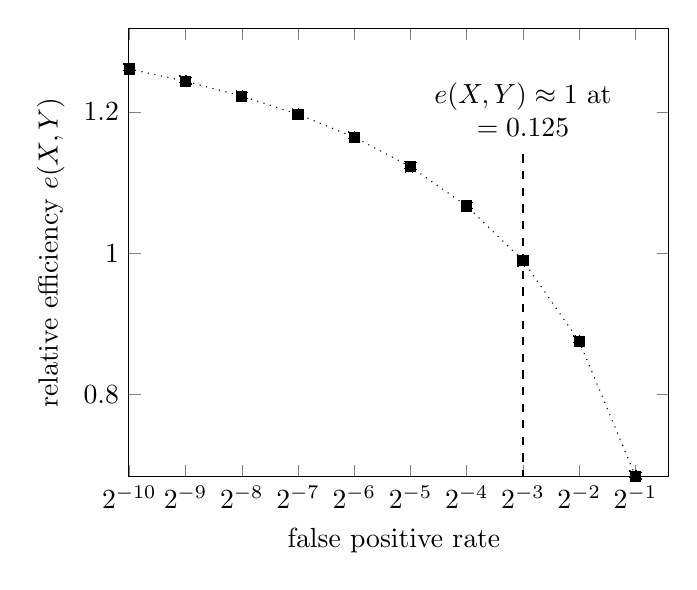
\begin{tikzpicture}
\begin{axis}[
    log basis x=2,
    xmode=log,
    ymin=.684,
    xmin=0.00097,
    xmax=.75,
    xlabel={false positive rate $\fprate$},
    ylabel={relative efficiency $e(X,Y)$},
    legend pos=north west,
    ]
    \addplot[dashed] coordinates {(0.125,0) (0.125,1.15)};
    \addplot[dotted,mark=square*] table
    {
        7.5231638e-37   1.42556
        8.6736174e-19   1.40882
        9.3132257e-10   1.3765
        9.53674316e-7   1.34563
        0.000976563     1.26086
        0.00195313      1.24351
        0.00390625      1.22254
        0.0078125       1.19676
        0.015625        1.16435
        0.03125         1.12256
        0.0625          1.06694
        0.125           0.989713
        0.25            0.875478
        0.5             0.684375
    };
    \node[label={$e(X,Y) \approx 1$ at}] at (axis cs:0.125,1.175) {};
    \node[label={$\fprate = 0.125$}] at (axis cs:0.125,1.1375) {};
  \end{axis}
\end{tikzpicture}
\end{figure}

The bit length of an object $x$ is denoted by
\begin{equation}
    \BL(x)\,,
\end{equation}
e.g., the bit length of any $x \in \BitSet^*_n$ is given by $\BL(x) = n$. The relative space efficiency metric is given by the following definition.
\begin{definition}
The relative space efficiency of a data structure $X$ to a data structure $Y$ is given by the ratio of the bit length of $Y$ to the bit length of $X$ as given by
\begin{equation}
    e(X,Y)=\frac{\BL(Y)}{\BL(X)}\,,
\end{equation}
where $\BL$ is the bit length function. There are three possibilities:
\begin{enumerate}
    \item $\RE(X,Y) < 1 \iff X$ is less efficient than $Y$.
    \item $\RE(X,Y) = 1 \iff X$ and $Y$ are equally efficient.
    \item $\RE(X,Y) > 1 \iff X$ is more efficient than $Y$.
\end{enumerate}
\end{definition}

The \emph{absolute} space efficiency of an approximate set $X$ with a false positive rate $\fprate$ is given by
\begin{equation}
    \AE\!(X) = e(X,-\log_2 \fprate)\,.
\end{equation}
An asymptotically optimal space-efficient data structure has an absolute efficiency that goes to $1$ as the cardinality $m$ of the set being approximated goes to $\infty$. The absolute efficiency of the \gls{gls-phf} is not asymptotically optimal since it has an asymptotic limit less than $1$ that is a function of the false positive rate $\fprate$ as shown in \cref{fig:abs_eff}. However, as $\fprate$ goes to $0$ the absolute efficiency goes to $1$.

\paragraph{Comparisons to the \emph{\gls{gls-blf}}.}
The \gls{gls-phf} is most suitable as an immutable data structure. It is optimized for read-many, write-once usage patterns. Once it is constructed, only on the order of
\begin{equation}
    \mathcal{O} \left( 1 \right)
\end{equation}
hash functions need to be computed to test an element for membership. The Bloom filter is suitable as a mutable data structure; elements may be inserted into it at any point at a cost of increasing the false positive rates. However, it requires computing on the order of
\begin{equation}
    \mathcal{O}\left(-\log \fprate\right)
\end{equation}
hash functions per membership test.

The \emph{Bloom filter} has an expected encoding size given approximately by
\begin{equation}
    -1.44 \log_2 \fprate \; \si{bits \per element}\,.
\end{equation}
The absolute efficiency of the \gls{gls-blf} is approximately $\ln 2 \approx 0.69$.

The relative efficiency of the \gls{gls-phf} to the \gls{gls-blf} is a function of the false positive rate $\fprate$ as shown in \cref{fig:rel_eff_bf_PHF,fig:abs_eff}. For this idealized construction, the break-even point is $\fprate \approx 2^{-3}$: if $\fprate < 2^{-3}$, the \gls{gls-phf} is more space efficient; otherwise the \gls{gls-blf} is more space efficient. As $\fprate$ goes to $0$, the relative efficiency of the \gls{gls-phf} to the \gls{gls-blf} goes to $1.44$.

\subsection{Entropy}
If the load factor is known, the cardinality of $\Set{S} \subset \PASet{S}$ is given by
\begin{equation}
    \Card{\Set{S}} = N r\,.
\end{equation}

If the load factor is not known, then the cardinality may be probabilistically estimated from the bit length, since the expected bit length is an increasing function of the cardinality. The randomness in the bit length comes entirely from the search for a perfect hash seed: by \cref{eq:perfect_hash_prob} each seed succeeds independently with probability $P(m, N)$, so the number of seeds examined is geometric and the seed length is its base-two logarithm. Combining the resulting expected seed cost (\cref{thm:mPHF_size}) with the fixed fingerprint width gives the concentration result below; we do not need the exact distribution of the seed length to estimate the cardinality, only its mean.

If the bit matrix of fingerprints $\matrx{V}$ has $m$ rows and $M$ columns, then $\Card{\Set{S}} \leq m$ and the expected false positive rate is $\fprate=2^{-M}$.

\begin{theorem}
\label{thm:max_entropy_coder}
The random bit string that codes the \gls{gls-phf} is a \emph{maximum entropy} coder for the \emph{positive Bernoulli set} abstract data type: conditioned on the cardinality $m$ and the false positive rate $\fprate$, every bit of the code is an independent fair coin.
\end{theorem}
\begin{proof}
A binary string has maximum entropy when its bits are independent and each is $\berdist(1/2)$. The \gls{gls-phf} code is the pair $\Tuple{\matrx{V}, n}$ of the fingerprint matrix and the perfect-hash seed. Each entry of $\matrx{V}$ is $\trunc(\ro(x), M)$ for a distinct member $x$; by \cref{asm:ro} the random oracle $\ro$ is uniform on $\BitSet^M$ and independent across distinct inputs, so the $m M$ fingerprint bits are i.i.d.\ $\berdist(1/2)$. The seed $n$ is the index of the first injective placement among i.i.d.\ uniform draws, so its bits are likewise uniform. Hence, given $m$ and $\fprate$, no further structure is imposed beyond the Bernoulli axioms, and the code attains the maximum conditional entropy. This is the discrete analogue of the entropy-map optimality of \cref{thm:approx_l_b}: the code carries no information about \emph{which} elements are members, only the minimum needed to realize the prescribed rate.
\end{proof}

Prior to any membership test, the only information the code carries about $\Set{S}$ is its cardinality, through the distribution of the bit length $\RV{N}$, which concentrates around
\begin{equation}
\label{eq:phf_expected_bits}
    \Expect{\RV{N}} = -m \log_2 \fprate + m \log_2 e\,,
\end{equation}
by \cref{cor:mPHF_size} (the minimal case; the load-factor-$r$ case replaces $\log_2 e$ with the bound of \cref{thm:mPHF_size}).

\begin{theorem}
\label{thm:phf_mom_estimator}
A \emph{method-of-moments} estimator of the cardinality of an approximated set represented by a minimal \gls{gls-phf} is given by
\begin{equation}
    \hat{m} = \frac{\BL\!\left(\PASet{S}\right)}{-\log_2 \fprate + \log_2 e}\,,
\end{equation}
where $\BL$ is the bit length function and $\fprate$ is the \emph{\gls{gls-fprate}}.
\end{theorem}
\begin{proof}
The \emph{expected} bit length is given by \cref{eq:phf_expected_bits},
\begin{equation*}
    \Expect{\RV{N}} = -m \log_2 \fprate + m \log_2 e\,,
    \tag{\ref{eq:phf_expected_bits} revisited}
\end{equation*}
where $m$ is the cardinality of the approximated set. The method-of-moments estimator is obtained by equating the observed bit length of the \gls{gls-phf} to this expectation,
\begin{equation}
    \BL(\PASet{S}) = -\hat{m} \log_2 \fprate + \hat{m} \log_2 e\,,
\end{equation}
and solving for $\hat{m}$, which yields the estimator
\begin{equation}
    \hat{m} = \frac{\BL(\PASet{S})}{-\log_2 \fprate + \log_2 e}\,.
\end{equation}
\end{proof}
When the bit matrix is available, there is a simpler method: count the number of rows in the matrix $\matrx{V}$.

We made trade space complexity for entropy if desired. For instance, if we find a bit string of a length around $t > -m \log_2 \fprate$ that codes the \gls{gls-phf}, then an estimate of the cardinality is given by
\begin{equation}
    \hat{\Card{\Set{S}}} = -\frac{t}{\log_2 \fprate}\,.
\end{equation}
Thus, without knowing how $t$ was chosen, we can only infer that the approximated set has a cardinality approximately between $0$ and $-\frac{t}{\log_2 \fprate}$, which has an approximate entropy of $\log_2 t$. The coding efficiency is now given by
\begin{equation}
    0 < \frac{m}{t} \leq 1\,,
\end{equation}
which is the \emph{maximum} efficiency possible for an approximate set with $\log_2 t$ entropy for the cardinality.

\end{document}
